\documentclass[]{book}
\usepackage{lmodern}
\usepackage{amssymb,amsmath}
\usepackage{ifxetex,ifluatex}
\usepackage{fixltx2e} % provides \textsubscript
\ifnum 0\ifxetex 1\fi\ifluatex 1\fi=0 % if pdftex
  \usepackage[T1]{fontenc}
  \usepackage[utf8]{inputenc}
\else % if luatex or xelatex
  \ifxetex
    \usepackage{mathspec}
  \else
    \usepackage{fontspec}
  \fi
  \defaultfontfeatures{Ligatures=TeX,Scale=MatchLowercase}
\fi
% use upquote if available, for straight quotes in verbatim environments
\IfFileExists{upquote.sty}{\usepackage{upquote}}{}
% use microtype if available
\IfFileExists{microtype.sty}{%
\usepackage{microtype}
\UseMicrotypeSet[protrusion]{basicmath} % disable protrusion for tt fonts
}{}
\usepackage[margin=1in]{geometry}
\usepackage{hyperref}
\hypersetup{unicode=true,
            pdftitle={Análise de Dados Amostrais Complexos},
            pdfauthor={Djalma Pessoa e Pedro Nascimento Silva},
            pdfborder={0 0 0},
            breaklinks=true}
\urlstyle{same}  % don't use monospace font for urls
\usepackage{natbib}
\bibliographystyle{apalike}
\usepackage{color}
\usepackage{fancyvrb}
\newcommand{\VerbBar}{|}
\newcommand{\VERB}{\Verb[commandchars=\\\{\}]}
\DefineVerbatimEnvironment{Highlighting}{Verbatim}{commandchars=\\\{\}}
% Add ',fontsize=\small' for more characters per line
\usepackage{framed}
\definecolor{shadecolor}{RGB}{248,248,248}
\newenvironment{Shaded}{\begin{snugshade}}{\end{snugshade}}
\newcommand{\KeywordTok}[1]{\textcolor[rgb]{0.13,0.29,0.53}{\textbf{{#1}}}}
\newcommand{\DataTypeTok}[1]{\textcolor[rgb]{0.13,0.29,0.53}{{#1}}}
\newcommand{\DecValTok}[1]{\textcolor[rgb]{0.00,0.00,0.81}{{#1}}}
\newcommand{\BaseNTok}[1]{\textcolor[rgb]{0.00,0.00,0.81}{{#1}}}
\newcommand{\FloatTok}[1]{\textcolor[rgb]{0.00,0.00,0.81}{{#1}}}
\newcommand{\ConstantTok}[1]{\textcolor[rgb]{0.00,0.00,0.00}{{#1}}}
\newcommand{\CharTok}[1]{\textcolor[rgb]{0.31,0.60,0.02}{{#1}}}
\newcommand{\SpecialCharTok}[1]{\textcolor[rgb]{0.00,0.00,0.00}{{#1}}}
\newcommand{\StringTok}[1]{\textcolor[rgb]{0.31,0.60,0.02}{{#1}}}
\newcommand{\VerbatimStringTok}[1]{\textcolor[rgb]{0.31,0.60,0.02}{{#1}}}
\newcommand{\SpecialStringTok}[1]{\textcolor[rgb]{0.31,0.60,0.02}{{#1}}}
\newcommand{\ImportTok}[1]{{#1}}
\newcommand{\CommentTok}[1]{\textcolor[rgb]{0.56,0.35,0.01}{\textit{{#1}}}}
\newcommand{\DocumentationTok}[1]{\textcolor[rgb]{0.56,0.35,0.01}{\textbf{\textit{{#1}}}}}
\newcommand{\AnnotationTok}[1]{\textcolor[rgb]{0.56,0.35,0.01}{\textbf{\textit{{#1}}}}}
\newcommand{\CommentVarTok}[1]{\textcolor[rgb]{0.56,0.35,0.01}{\textbf{\textit{{#1}}}}}
\newcommand{\OtherTok}[1]{\textcolor[rgb]{0.56,0.35,0.01}{{#1}}}
\newcommand{\FunctionTok}[1]{\textcolor[rgb]{0.00,0.00,0.00}{{#1}}}
\newcommand{\VariableTok}[1]{\textcolor[rgb]{0.00,0.00,0.00}{{#1}}}
\newcommand{\ControlFlowTok}[1]{\textcolor[rgb]{0.13,0.29,0.53}{\textbf{{#1}}}}
\newcommand{\OperatorTok}[1]{\textcolor[rgb]{0.81,0.36,0.00}{\textbf{{#1}}}}
\newcommand{\BuiltInTok}[1]{{#1}}
\newcommand{\ExtensionTok}[1]{{#1}}
\newcommand{\PreprocessorTok}[1]{\textcolor[rgb]{0.56,0.35,0.01}{\textit{{#1}}}}
\newcommand{\AttributeTok}[1]{\textcolor[rgb]{0.77,0.63,0.00}{{#1}}}
\newcommand{\RegionMarkerTok}[1]{{#1}}
\newcommand{\InformationTok}[1]{\textcolor[rgb]{0.56,0.35,0.01}{\textbf{\textit{{#1}}}}}
\newcommand{\WarningTok}[1]{\textcolor[rgb]{0.56,0.35,0.01}{\textbf{\textit{{#1}}}}}
\newcommand{\AlertTok}[1]{\textcolor[rgb]{0.94,0.16,0.16}{{#1}}}
\newcommand{\ErrorTok}[1]{\textcolor[rgb]{0.64,0.00,0.00}{\textbf{{#1}}}}
\newcommand{\NormalTok}[1]{{#1}}
\usepackage{longtable,booktabs}
\usepackage{graphicx,grffile}
\makeatletter
\def\maxwidth{\ifdim\Gin@nat@width>\linewidth\linewidth\else\Gin@nat@width\fi}
\def\maxheight{\ifdim\Gin@nat@height>\textheight\textheight\else\Gin@nat@height\fi}
\makeatother
% Scale images if necessary, so that they will not overflow the page
% margins by default, and it is still possible to overwrite the defaults
% using explicit options in \includegraphics[width, height, ...]{}
\setkeys{Gin}{width=\maxwidth,height=\maxheight,keepaspectratio}
\IfFileExists{parskip.sty}{%
\usepackage{parskip}
}{% else
\setlength{\parindent}{0pt}
\setlength{\parskip}{6pt plus 2pt minus 1pt}
}
\setlength{\emergencystretch}{3em}  % prevent overfull lines
\providecommand{\tightlist}{%
  \setlength{\itemsep}{0pt}\setlength{\parskip}{0pt}}
\setcounter{secnumdepth}{5}
% Redefines (sub)paragraphs to behave more like sections
\ifx\paragraph\undefined\else
\let\oldparagraph\paragraph
\renewcommand{\paragraph}[1]{\oldparagraph{#1}\mbox{}}
\fi
\ifx\subparagraph\undefined\else
\let\oldsubparagraph\subparagraph
\renewcommand{\subparagraph}[1]{\oldsubparagraph{#1}\mbox{}}
\fi

%%% Use protect on footnotes to avoid problems with footnotes in titles
\let\rmarkdownfootnote\footnote%
\def\footnote{\protect\rmarkdownfootnote}

%%% Change title format to be more compact
\usepackage{titling}

% Create subtitle command for use in maketitle
\newcommand{\subtitle}[1]{
  \posttitle{
    \begin{center}\large#1\end{center}
    }
}

\setlength{\droptitle}{-2em}
  \title{Análise de Dados Amostrais Complexos}
  \pretitle{\vspace{\droptitle}\centering\huge}
  \posttitle{\par}
  \author{Djalma Pessoa e Pedro Nascimento Silva}
  \preauthor{\centering\large\emph}
  \postauthor{\par}
  \predate{\centering\large\emph}
  \postdate{\par}
  \date{2017-09-02}

\usepackage{booktabs}
% \usepackage[brazil]{babel}
% \newtheorem{example}{Exemplo}
% \numberwithin{example}{chapter}
% \newtheorem{remark}{Observação}
% \numberwithin{remark}{chapter}
% \newtheorem{definition}{Definição}
% \numberwithin{definition}{chapter}

\usepackage{amsthm}
\newtheorem{theorem}{Teorema}[chapter]
\newtheorem{lemma}{Lema}[chapter]
\theoremstyle{definition}
\newtheorem{definition}{Definição}[chapter]
\newtheorem{corollary}{Corolário}[chapter]
\newtheorem{proposition}{Proposição}[chapter]
\theoremstyle{definition}
\newtheorem{example}{Exemplo}[chapter]
\theoremstyle{remark}
\newtheorem*{remark}{Observação }
\let\BeginKnitrBlock\begin \let\EndKnitrBlock\end
\begin{document}
\maketitle

{
\setcounter{tocdepth}{1}
\tableofcontents
}
\chapter*{Prefácio}\label{prefacio}
\addcontentsline{toc}{chapter}{Prefácio}

\chapter{Introdução}\label{introduc}

\section{Motivação}\label{motivacao}

Este livro trata de problema de grande importância para os usuários de
dados obtidos através de pesquisas amostrais por agências produtoras de
informações estatísticas. Tais dados são comumente utilizados em
análises descritivas envolvendo o cálculo de estimativas para totais,
proporções, médias e razões, nas quais, em geral, são devidamente
considerados os pesos distintos das observações e o planejamento da
amostra que lhes deu origem.

Outro uso destes dados, denominado secundário, é a construção e ajuste
de modelos, feita geralmente por analistas que trabalham fora das
agências produtoras dos dados. Neste caso, o foco é, essencialmente,
estabelecer a natureza de relações ou associações entre variáveis. Para
isto, a estatística clássica conta com um arsenal de ferramentas de
análise, já incorporado aos principais pacotes estatísticos disponíveis.
O uso destes pacotes se faz, entretanto, sob condições que não refletem
a complexidade usualmente envolvida nas pesquisas amostrais de
populações finitas. Em geral, partem de hipóteses básicas que só são
válidas quando os dados são obtidos através de amostras aleatórias
simples com reposição (AASC). Tais pacotes estatísticos não consideram
os seguintes aspectos relevantes no caso de amostras complexas:

i.) \textbf{probabilidades distintas de seleção das unidades};

ii.) \textbf{conglomeração das unidades};

iii.) \textbf{estratificação};

iv.) \textbf{calibração ou imputação para não-resposta e outros
ajustes}.

As estimativas pontuais de parâmetros da população ou de modelos são
influenciadas por pesos distintos das observações. Além disso, as
estimativas de variância (ou da precisão dos estimadores) são
influenciadas pela conglomeração, estratificação e pesos, ou no caso de
não resposta, também por eventual imputação de dados faltantes. Ao
ignorar estes aspectos, os pacotes tradicionais de análise podem
produzir estimativas incorretas das variâncias das estimativas pontuais.

A seguir vamos apresentar um exemplo de uso de dados de uma pesquisa
amostral real para ilustrar como os pontos i) a iv) acima mencionados
afetam a inferência sobre quantidades descritivas populacionais tais
como médias, proporções, razões e totais.

\BeginKnitrBlock{example}
\protect\hypertarget{ex:distppv}{}{\label{ex:distppv}}Distribuição dos pesos
da amostra da PPV
\EndKnitrBlock{example}

Os dados deste exemplo são relativos à distribuição dos pesos na amostra
da Pesquisa sobre Padrões de Vida (PPV), realizada pelo IBGE nos anos
1996-97. \citep{albieri} descrevem resumidamente a Pesquisa sobre
Padrões de Vida (PPV), que foi realizada nas Regiões Nordeste e Sudeste
do País, considerando 10 estratos geográficos, a saber: Região
Metropolitana de Fortaleza, Região Metropolitana de Recife, Região
Metropolitana de Salvador, restante da área urbana do Nordeste, restante
da área rural do Nordeste, Região Metropolitana de Belo Horizonte,
Região Metropolitana do Rio de Janeiro, Região Metropolitana de São
Paulo, restante da área urbana do Sudeste e restante da área rural do
Sudeste.

O plano amostral empregado na seleção da amostra da PPV foi de dois
estágios, com estratificação das unidades primárias de amostragem (no
caso os setores censitários da base geográfica do IBGE conforme usada
para o Censo Demográfico de 1991), seleção destes setores com
probabilidade proporcional ao tamanho, e seleção aleatória das unidades
de segundo estágio (domicílios). O tamanho da amostra para cada estrato
geográfico foi fixado em 480 domicílios, e o número de setores
selecionados foi fixado em 60, com 8 domicílios selecionados em cada
setor. A exceção ficou por conta dos estratos que correspondem ao
restante da área rural de cada Região, onde foram selecionados 30
setores e 16 domicílios por setor, em função da dificuldade de acesso a
esses setores, o que implicaria em aumento de custo da coleta.

Os setores de cada um dos 10 estratos geográficos foram subdivididos em
3 estratos de acordo com a renda média mensal do chefe do domicílio por
setor, perfazendo um total de 30 estratos geográficos versus renda. Em
seguida foi feita uma alocação proporcional, com base no número de
domicílios particulares permanentes ocupados do estrato de renda no
universo de cada estrato geográfico, obtidos pelo Censo de 1991. No
final foram obtidos 554 setores na amostra, distribuídos tal como revela
a Tabela \ref{tab:numset}.

\begin{table}

\caption{\label{tab:numset}Número de setores na população e na amostra, por estrato geográfico}
\centering
\begin{tabular}[t]{lcclcclcc}
\toprule
Estrato & População & Amostra\\
\midrule
RM Fortaleza & 2263 & 62\\
RM Recife & 2309 & 61\\
RM Salvador & 2186 & 61\\
Restante Nordeste Urbano & 15057 & 61\\
Restante Nordeste Rural & 23711 & 33\\
\addlinespace
RM Belo Horizonte & 3283 & 62\\
RM Rio de Janeiro & 10420 & 61\\
RM São Paulo & 14931 & 61\\
Restante Sudeste Urbano & 25855 & 61\\
Restante Sudeste Rural & 12001 & 31\\
Total & 112016 & 554\\
\bottomrule
\end{tabular}
\end{table}

A Tabela \ref{tab:dispesos} apresenta um resumo das distribuições dos
pesos amostrais para as Regiões Nordeste (5 estratos geográficos) e
Sudeste (5 estratos geográficos) separadamente e para o conjunto da
amostra da PPV.

\begin{table}

\caption{\label{tab:dispesos}Distribuição dos pesos da amostra da PPV}
\centering
\begin{tabular}[t]{lccccclccccclccccclccccclccccclccccc}
\toprule
Região & Mínimo & Q1 & Mediana & Q3 & Máximo\\
\midrule
Nordeste & 724 & 1194 & 1556 & 6937 & 15348\\
Sudeste & 991 & 2789 & 5429 & 9509 & 29234\\
Nordeste\_Sudeste & 724 & 1403 & 3785 & 8306 & 29234\\
\bottomrule
\end{tabular}
\end{table}

No cálculo dos pesos foram consideradas as probabilidades de inclusão
dos elementos na amostra bem como correções devido a não-resposta.
Contudo, a grande variabilidade dos pesos amostrais da PPV é devida à
variabilidade das probabilidades de inclusão na amostra, ilustrando
desta forma o ponto i) citado anteriormente nesta seção.

Na análise de dados desta pesquisa, deve-se considerar que há elementos
da amostra com pesos bem distintos. Por exemplo, a razão entre o maior e
o menor peso é cerca de 40 vezes. Tais pesos são utilizados para
\texttt{expandir} os dados, multiplicando-se cada observação pelo seu
respectivo peso. Assim, por exemplo, para \texttt{estimar} quantos
elementos \texttt{da\ população} pertencem a determinado conjunto
(domínio), basta somar os pesos dos elementos da amostra que pertencem a
este conjunto. É possível ainda incorporar os pesos, de maneira simples
e natural, quando estimamos medidas descritivas simples da população
tais como totais, médias, proporções, razões, etc.

Por outro lado, quando utilizamos a amostra para estudos analíticos, as
opções padrão disponíveis nos pacotes estatísticos usuais para levar em
conta os pesos distintos das observações são apropriadas somente para
observações independentes e identicamente distribuídas (IID). Por
exemplo, os procedimentos padrão disponíveis para estimar a média
populacional permitem utilizar pesos distintos das observações
amostrais, mas tratariam tais pesos como se fossem frequências de
observações repetidas na amostra, e portanto interpretariam a soma dos
pesos como tamanho amostral, situação que na maioria das vezes gera
inferências incorretas sobre a precisão das estimativas, pois o tamanho
da amostra é muito menor que a soma dos pesos amostrais usualmente
encontrados nos arquivos de microdados de pesquisas disseminados por
agências de estatísticas oficiais. Em tais pesquisas, a opção mais
freqüente é disseminar pesos que somados estimam o total de unidades
\texttt{da\ população}.

Além disso, a variabilidade dos pesos para distintas observações
amostrais produz impactos tanto na estimação pontual quanto na estimação
das variâncias dessas estimativas, que sofre ainda influência da
conglomeração e estratificação - pontos ii) e iii) mencionados
anteriormente.

Para exemplificar o impacto de ignorar os pesos e o plano amostral ao
estimar quantidades descritivas populacionais, tais como totais, médias,
proporções e razões, calculamos estimativas de quantidades desses
diferentes tipos usando a amostra da PPV juntamente com estimativas das
respectivas variâncias. Essas estimativas de variâncias foram calculadas
sob duas estratégias: considerando amostragem aleatória simples
(portanto ignorando o plano amostral efetivamente adotado), e
considerando o plano amostral da pesquisa e os pesos diferenciados das
unidades. A razão entre as estimativas de variância obtidas sob o plano
amostral verdadeiro e sob amostragem aleatória simples foi calculada
para cada uma das estimativas consideradas usando a library
\texttt{survey} do R \citep{R-survey} . Essa razão fornece uma medida do
efeito de ignorar o plano amostral . Os resultados das estimativas
ponderadas e variâncias considerando o plano amostral são apresentados
na Tabela \ref{tab:epas} , juntamente com as medidas dos efeitos de
plano amostral (EPA). Exemplos de utilização da library \texttt{survey}
para obtenção de estimativas apresentadas na \ref{tab:epas} estão na
Seção \ref{epa}. As outras estimativas da Tabela \ref{tab:epas} podem
ser obtidas de maneira análoga.

Na Tabela \ref{tab:epas} apresentamos as estimativas dos seguintes
parâmetros populacionais:

\begin{enumerate}
\def\labelenumi{\arabic{enumi}.}
\tightlist
\item
  Número médio de pessoas por domicílio;
\item
  \% de domicílios alugados;
\item
  Número total de pessoas que avaliaram seu estado de de saúde como
  ruim;
\item
  Total de analfabetos de 7 a 14 anos;
\item
  Total de analfabetos de mais de 14 anos;
\item
  \% de analfabetos de 7 a 14 anos;
\item
  \% de analfabetos de mais de 14 anos;
\item
  Total de mulheres de 12 a 49 anos que tiveram filhos;
\item
  Total de mulheres de 12 a 49 anos que tiveram filhos vivos; 10.Total
  de mulheres de 12 a 49 anos que tiveram filhos mortos;
\item
  Número médio de filhos tidos por mulheres de 12 a 49 anos;
\item
  Razão de dependência.
\end{enumerate}

\begin{table}

\caption{\label{tab:epas}Estimativas de Efeitos de Plano Amostral (EPAs)
para variáveis selecionadas da PPV - Região Sudeste}
\centering
\begin{tabular}[t]{rrrrrrrrr}
\toprule
Estimativa & DP & EPA\\
\midrule
3.62 & 0.05 & 2.64\\
10.70 & 1.15 & 2.97\\
1208123.00 & 146681.00 & 3.37\\
1174220.00 & 127982.00 & 2.64\\
4792344.00 & 318877.00 & 4.17\\
\addlinespace
11.87 & 1.18 & 2.46\\
10.87 & 0.67 & 3.86\\
10817590.00 & 322947.00 & 2.02\\
10804511.00 & 323182.00 & 3.02\\
709145.00 & 87363.00 & 2.03\\
\addlinespace
1.39 & 0.03 & 1.26\\
0.53 & 0.01 & 1.99\\
\bottomrule
\end{tabular}
\end{table}

Como se pode observar da quarta coluna da Tabela \ref{tab:epas}, os
valores do efeito do plano amostral variam de um modesto 1,26 para o
número médio de filhos tidos por mulheres em idade fértil (12 a 49 anos
de idade) até um substancial 4,17 para o total de analfabetos entre
pessoas de mais de 14 anos. Nesse último caso, usar a estimativa de
variância como se o plano amostral fosse amostragem aleatória simples
implicaria em subestimar consideravelmente a variância da estimativa
pontual, que é mais que 4 vezes maior se consideramos o plano amostral
efetivamente utilizado.

Note que as variáveis e parâmetros cujas estimativas são apresentadas na
Tabela \ref{tab:epas} não foram escolhidas de forma a acentuar os
efeitos ilustrados, mas tão somente para representar distintos
parâmetros (médias, razões, totais, proporções) e variáveis de
interesse. Os resultados apresentados para as estimativas de EPA
ilustram bem o cenário típico em pesquisas amostrais complexas: o
impacto do plano amostral sobre a inferência varia conforme a variável e
o tipo de parâmetro de interesse. Note ainda que à exceção do menor
valor, todas as demais estimativas de EPA apresentaram valores
superiores a 2.

\section{Objetivos do Livro}\label{objetivos-do-livro}

Este livro tem três objetivos principais:

\begin{enumerate}
\def\labelenumi{\arabic{enumi})}
\item
  \textbf{ilustrar e analisar o impacto das simplificações feitas ao
  utilizar pacotes usuais de análise de dados quando estes são
  provenientes de pesquisas amostrais complexas};
\item
  \textbf{apresentar uma coleção de métodos e recursos computacionais
  disponíveis para análise de dados amostrais complexos, equipando o
  analista para trabalhar com tais dados, reduzindo assim o risco de
  inferências incorretas};
\item
  \textbf{ilustrar o potencial analítico de muitas das pesquisas
  produzidas por agências de estatísticas oficiais para responder
  questões de interesse, mediante uso de ferramentas de análise
  estatística agora já bastante difundidas, aumentando assim o valor
  adicionado destas pesquisas}.
\end{enumerate}

Para alcançar tais objetivos, adota-se uma abordagem fortemente ancorada
na apresentação de exemplos de análises de dados obtidos em pesquisas
amostrais complexas, usando pacotes clássicos e também recursos do
pacote estatístico R (\url{http://www.r-project.org/}). A comparação dos
resultados das análises feitas das duas formas permite avaliar o impacto
de não se considerar os pontos i) a iv) anteriormente citados. O ponto
iv) não será tratado de forma completa neste texto. O leitor interessado
na análise de dados sujeitos a não-resposta pode consultar
\citep{kalton83a}, \citep{LR2002}, \citep{Rubin87}, \citep{SSW92}, ou
Schafer (1997), por exemplo.

\textbf{Estrutura do Livro}

O livro está organizado em catorze capítulos. Este primeiro capítulo
discute a motivação para estudar o assunto e apresenta uma ideia geral
dos objetivos e da estrutura do livro.

No segundo capítulo, procuramos dar uma visão das diferentes abordagens
utilizadas na análise estatística de dados de pesquisas amostrais
complexas. Apresentamos um referencial para inferência com ênfase no
\texttt{Modelo\ de\ Superpopulação} que incorpora, de forma natural,
tanto uma estrutura estocástica para descrever a geração dos dados
populacionais (modelo) como o plano amostral efetivamente utilizado para
obter os dados amostrais (plano amostral). As referências básicas para
seguir este capítulo são cap2 em \citep{Silva}, cap1 em \citep{SHS89} e
caps 1 e 2 em \citep{CHSK2003}.

Esse referencial tem evoluído ao longo dos anos como uma forma de
permitir a incorporação de idéias e procedimentos de análise e
inferência usualmente associados à Estatística Clássica à prática da
interpretação de dados provenientes de pesquisas amostrais. Apesar dessa
evolução, sua adoção não é livre de controvérsia e uma breve revisão
dessa discussão é apresentada no Capítulo \ref{refinf}.

No Capítulo \ref{capplanamo} apresentamos uma revisão sucinta, a título
de recordação, de alguns resultados básicos da Teoria de Amostragem,
requeridos nas partes subsequentes do livro. São discutidos os
procedimentos básicos para estimação de totais considerando o plano
amostral, e em seguida revistas algumas técnicas para estimação de
variâncias úteis para o caso de estatísticas complexas, tais como razões
e outras estatísticas requeridas na inferência analítica com dados
amostrais. As referências centrais para este capítulo são caps 2 e 3 em
\citep{SSW92}, \citep{W85} e \citep{cochran}.

No Capítulo \ref{epa} introduzimos o conceito de
\texttt{Efeito\ do\ Plano\ Amostral\ (EPA)}, que permite avaliar o
impacto de ignorar a estruturação dos dados populacionais ou do plano
amostral sobre a estimativa da variância de um estimador. Para isso,
comparamos o estimador da variância apropriado para dados obtidos por
amostragem aleatória simples (hipótese de AAS) com o valor esperado
deste mesmo estimador sob a distribuição de aleatorização induzida pelo
plano amostral efetivamente utilizado (plano amostral verdadeiro). Aqui
a referência principal foi o livro \citep{SHS89}, complementado com o
texto de \citep{lethonen}.

No Capítulo \ref{ajmodpar} estudamos a questão do uso de pesos ao
analisar dados provenientes de pesquisas amostrais complexas, e
introduzimos um método geral, denominado
\texttt{Método\ de\ Máxima\ Pseudo\ Verossimilhança(MPV)}, para
incorporar os pesos e o plano amostral na obtenção não só de estimativas
de parâmetros dos modelos regulares de interesse, como também das
variâncias dessas estimativas. As referências básicas utilizadas nesse
capítulo foram \citep{SHS89}, \citep{Pfeff}, \citep{binder83} e cap.6 em
\citep{Silva}.

O Capítulo \ref{modreg} trata da obtenção de
\texttt{Estimadores\ de\ Máxima\ Pseudo-Verossimilhança\ (EMPV)} e da
respectiva matriz de covariância para os parâmetros em modelos de
regressão linear e de regressão logística, quando os dados vêm de
pesquisas amostrais complexas. Apresentamos um exemplo de aplicação com
dados do Suplemento Trabalho da Pesquisa Nacional por Amostra de
Domicílios (PNAD) de 90, onde ajustamos um modelo de regressão
logística. Neste exemplo, são feitas comparações entre resultados de
ajustes obtidos através de um programa especializado, a library
\texttt{survey} \citep{R-survey}, e através de um programa de uso geral,
a library \texttt{glm} do R. As referências centrais são cap6 em
\citep{Silva} e Binder(1983), além de \citep{Pessoa}.

Os Capítulos \ref{testqualajust} e \ref{testetab2} tratam da análise de
dados categóricos com ênfase na adaptação dos testes clássicos para
proporções, de independência e de homogeneidade em tabelas de
contingência, para dados provenientes de pesquisas amostrais complexas.
Apresentamos correções das estatísticas clássicas e a estatística de
Wald baseada no plano amostral. As referências básicas usadas nesses
capítulos foram os livros cap. 4, \citep{SHS89} e cap. 7
\citep{lethonen}. Também são apresentadas as idéias básicas de como
efetuar ajuste de modelos log-lineares a dados de frequências em tabelas
de múltiplas entradas.

O Capítulo \ref{estimacao-de-densidades} trata da estimação de
densidades e funções de distribuição, ferramentas que tem assumido
importância cada dia maior com a maior disponibilidade de microdados de
pesquisas amostrais para analistas fora das agências produtoras.

O Capítulo \ref{modelos-hierarquicos} trata da estimação e ajuste de
modelos hierárquicos considerando o plano amostral. Modelos hierárquicos
(ou modelos multinível) têm sido bastante utilizados para explorar
situações em que as relações entre variáveis de interesse em uma certa
população de unidades elementares (por exemplo, crianças em escolas,
pacientes em hospitais, empregados em empresas, moradores em regiões,
etc.) são afetadas por efeitos de grupos determinados ao nível de
unidades conglomeradas (os grupos). Ajustar e interpretar tais modelos é
tarefa mais difícil que o mero ajuste de modelos lineares mesmo em casos
onde os dados são obtidos de forma exaustiva, mas ainda mais complicada
quando se trata de dados obtidos através de pesquisas amostrais
complexas. Várias alternativas de métodos para ajuste de modelos
hierárquicos estão disponíveis, e este capítulo apresenta uma revisão de
tais abordagens, ilustrando com aplicações a dados de pesquisas
amostrais de escolares.

O Capítulo \ref{nao-resposta} trata da não resposta e suas conseqüências
sobre a análise de dados. As abordagens de tratamento usuais,
reponderação e imputação, são descritas de maneira resumida, com
apresentação de alguns exemplos ilustrativos, e referências à ampla
literatura existente sobre o assunto. Em seguida destacamos a
importância de considerar os efeitos da não-resposta e dos tratamentos
compensatórios aplicados nas análises dos dados resultantes, destacando
em particular as ferramentas disponíveis para a estimação de variâncias
na presença de dados incompletos tratados mediante reponderação e/ou
imputação.

O Capítulo \ref{diagnostico-de-ajuste-de-modelo} trata de assunto ainda
emergente: diagnósticos do ajuste de modelos quando os dados foram
obtidos de amostras complexas. A literatura sobre o assunto ainda é
incipiente, mas o assunto é importante e procura-se estimular sua
investigação com a revisão do estado da arte no assunto.

O Capítulo \ref{agregdesag} discute algumas formas alternativas de
analisar dados de pesquisas complexas, contrapondo algumas abordagens
distintas à que demos preferência nos capítulos anteriores, para dar aos
leitores condições de apreciar de forma crítica o material apresentado
no restante deste livro. Entre as abordagens discutidas, há duas
principais: a denominada \texttt{análise\ desagregada}, e a abordagem
denominada \texttt{obtenção\ \ do\ modelo\ amostral} proposta por
\citep{PKR}. A chamada \texttt{análise\ desagregada} incorpora
explicitamente na análise vários aspectos do plano amostral utilizado
através do emprego de modelos hierárquicos \citep{bryk}. Em contraste, a
abordagem adotada nos oito primeiros capítulos é denominada
\texttt{análise\ agregada}, e procura \texttt{eliminar} da análise
efeitos tais como conglomeração induzida pelo plano amostral,
considerando tais efeitos como \texttt{ruídos} ou fatores de perturbação
que \texttt{atrapalham} o emprego dos procedimentos clássicos de
estimação, ajuste de modelos e teste de hipóteses.

A abordagem de \texttt{obtenção\ do\ modelo\ amostral} parte de um
modelo de superpopulação e procura derivar o modelo amostral (ou que
valeria para as observações da amostra obtida) considerando modelos para
as probabilidades de inclusão dadas as variáveis auxiliares e as
variáveis resposta de interesse. Uma vez obtidos tais modelos, seu
ajuste prossegue por métodos convencionais tais como máxima
verossimilhança ou mesmo MCMC (Markov Chain Monte Carlo).

Por último, no Capítulo \ref{pacotes}, listamos alguns pacotes
computacionais especializados disponíveis para a análise de dados de
pesquisas amostrais complexas. Sem pretender ser exaustiva ou detalhada,
essa revisão dos pacotes procura também apresentar suas características
mais importantes. Vários destes programas podem ser adquiridos
gratuitamente via \texttt{internet}, nos endereços fornecidos de seus
produtores. Com isto pretendemos indicar aos leitores o caminho mais
curto para permitir a implementação prática das técnicas e métodos aqui
discutidos.

Uma das características que procuramos dar ao livro foi o emprego de
exemplos com dados reais, retirados principalmente da experiência do
IBGE com pesquisas amostrais complexas. Embora a experiência de fazer
inferência analítica com dados desse tipo seja ainda incipiente no
Brasil, acreditamos ser fundamental difundir essas idéias para alimentar
um processo de melhoria do aproveitamento dos dados das inúmeras
pesquisas realizadas pelo IBGE e instituições congêneres, que permita ir
além da tradicional estimação de médias, totais, proporções e razões.
Esperamos com esse livro fazer uma contribuição a esse processo.

Uma dificuldade em escrever um livro como este vem do fato de que não é
possível começar do zero: é preciso assumir algum conhecimento prévio de
idéias e conceitos necessários à compreensão do material tratado.
Procuramos tornar o livro acessível para um estudante de fim de curso de
graduação em Estatística. Por essa razão optamos por não apresentar
provas de resultados e sempre que possível, apresentar os conceitos e
idéias de maneira intuitiva, juntamente com uma discussão mais formal
para dar solidez aos resultados apresentados. As provas de vários dos
resultados aqui discutidos se restringem a material disponível apenas em
artigos em periódicos especializados estrangeiros e portanto, são de
acesso mais difícil. Ao leitor em busca de maior detalhamento e rigor,
sugerimos consultar diretamente as inúmeras referências incluídas ao
longo do texto. Para um tratamento mais profundo do assunto, os livros
de \citep{SHS89} e \citep{CHSK2003} são as referências centrais a
pesquisar. Para aqueles querendo um tratamento ainda mais prático que o
nosso, o livro de \citep{lethonen} pode ser uma opção interessante.

\section{Laboratório de R do Capítulo 1.}\label{epa}

\BeginKnitrBlock{example}
\protect\hypertarget{ex:unnamed-chunk-1}{}{\label{ex:unnamed-chunk-1}}Utilização
da library survey do R para estimar totais e razões na PPV
\EndKnitrBlock{example} Os exemplos a seguir utilizam dados da Pesquisa
de Padrões de Vida (\texttt{PPV}) de 2004 do IBGE, cujo plano amostral
encontra-se descrito no Exemplo \ref{ex:distppv} . Inicialmente, vamos
ler os dados e definir variáveis de interesse por meio de transformação
das variáveis existentes.

\begin{Shaded}
\begin{Highlighting}[]
\CommentTok{# leitura dos dados}
\NormalTok{ppv1 <-}\StringTok{ }\KeywordTok{readRDS}\NormalTok{(}\StringTok{"~}\CharTok{\textbackslash{}\textbackslash{}}\StringTok{GitHub}\CharTok{\textbackslash{}\textbackslash{}}\StringTok{adac}\CharTok{\textbackslash{}\textbackslash{}}\StringTok{data}\CharTok{\textbackslash{}\textbackslash{}}\StringTok{ppv.rds"}\NormalTok{)}
\KeywordTok{library}\NormalTok{(survey)}
\end{Highlighting}
\end{Shaded}

Criação das variáveis analf1, analf2, faixa1 e faixa2:

\begin{Shaded}
\begin{Highlighting}[]
\NormalTok{ppv1 <-}\StringTok{ }\KeywordTok{transform}\NormalTok{(ppv1, }
\DataTypeTok{analf1 =} \NormalTok{((v04a01 ==}\StringTok{ }\DecValTok{2} \NormalTok{|}\StringTok{ }\NormalTok{v04a02 ==}\StringTok{ }\DecValTok{2}\NormalTok{) &}\StringTok{ }\NormalTok{(v02a08 >=}\StringTok{ }\DecValTok{7} \NormalTok{&}\StringTok{ }\NormalTok{v02a08 <=}\StringTok{ }\DecValTok{14}\NormalTok{)) *}\StringTok{ }\DecValTok{1}\NormalTok{, }
\DataTypeTok{analf2 =} \NormalTok{((v04a01 ==}\StringTok{ }\DecValTok{2} \NormalTok{|}\StringTok{ }\NormalTok{v04a02 ==}\StringTok{ }\DecValTok{2}\NormalTok{) &}\StringTok{ }\NormalTok{(v02a08 >}\DecValTok{14}\NormalTok{)) *}\StringTok{ }\DecValTok{1}\NormalTok{, }
\DataTypeTok{faixa1 =} \NormalTok{(v02a08 >=}\StringTok{ }\DecValTok{7} \NormalTok{&}\StringTok{ }\NormalTok{v02a08 <=}\StringTok{ }\DecValTok{14}\NormalTok{) *}\DecValTok{1}\NormalTok{, }
\DataTypeTok{faixa2 =} \NormalTok{(v02a08 >}\StringTok{ }\DecValTok{14}\NormalTok{) *}\StringTok{ }\DecValTok{1}\NormalTok{)}
\end{Highlighting}
\end{Shaded}

A seguir, mostramos a utilização da library \texttt{survey}
\citep{R-survey} do R para obter algumas estimativas da Tabela
\ref{tab:epas}. Vamos supor que os dados da pesquisa estão contidos no
data frame \texttt{ppv1}, que contém as variáveis que caracterizam o
plano amostral

\begin{itemize}
\tightlist
\item
  nsetor - conglomerados;
\item
  estratof - estratos;
\item
  pesof - pesos do plano amostral;
\end{itemize}

e variáveis de interesse tais como:

\begin{itemize}
\tightlist
\item
  regiao - regiões de abrangência: 1- Nordeste, 2- Sudeste;
\item
  analf1 - indicador de analfabeto na faixa etária de 7 a 14 anos;
\item
  analf2 - indicador de analfabeto na faixa etária acima de 14 anos;
\item
  faixa1 - indicador de idade entre 7 e 14 anos;
\item
  faixa2 - indicador de idade acima de 14 anos;
\end{itemize}

O passo fundamental para utilização da library \texttt{survey}
\citep{R-survey} é criar um objeto que guarde as informações relevantes
do plano amostral. Isso é feito por meio da função \texttt{svydesign()}.
As variáveis que definem estratos, conglomerados e pesos na \texttt{PPV}
são respectivamente, \texttt{estratof}, \texttt{nsetor} e
\texttt{pesof}. O objeto de desenho amostral, \texttt{ppv.des} incorpora
as informações do plano amostral adotado na \texttt{PPV}.

\begin{Shaded}
\begin{Highlighting}[]
\KeywordTok{library}\NormalTok{(survey)}
\NormalTok{ppv.des<-}\KeywordTok{svydesign}\NormalTok{(}\DataTypeTok{ids =} \NormalTok{~nsetor, }\DataTypeTok{strata =} \NormalTok{~estratof,}
\DataTypeTok{data =} \NormalTok{ppv1, }\DataTypeTok{nest =} \OtherTok{TRUE}\NormalTok{, }\DataTypeTok{weights =} \NormalTok{~pesof)}
\end{Highlighting}
\end{Shaded}

Como todos os exemplos a seguir serão relativos a estimativas na Região
Sudeste, vamos restringir o desenho a esse domínio:

\begin{Shaded}
\begin{Highlighting}[]
\NormalTok{ppv.se.des <-}\StringTok{ }\KeywordTok{subset}\NormalTok{(ppv.des, regiao ==}\StringTok{ }\DecValTok{2}\NormalTok{)}
\end{Highlighting}
\end{Shaded}

Para exemplificar, vamos estimar algumas características da população,
descritas na Tabela \ref{tab:epas}. Os totais das variáveis
\texttt{analf1} e \texttt{analf2} para a região Sudeste fornecem os
resultados nas linhas 4 e 5 da Tabela \ref{tab:epas}:

\begin{itemize}
\tightlist
\item
  totais de analfabetos nas faixas etárias de 7 a 14 anos e acima de 14
  anos.
\end{itemize}

\begin{Shaded}
\begin{Highlighting}[]
\KeywordTok{svytotal}\NormalTok{(~analf1, ppv.se.des, }\DataTypeTok{deff =} \OtherTok{TRUE}\NormalTok{)}
\end{Highlighting}
\end{Shaded}

\begin{verbatim}
##          total      SE   DEff
## analf1 1174220  127982 2.0543
\end{verbatim}

\begin{Shaded}
\begin{Highlighting}[]
\KeywordTok{svytotal}\NormalTok{(~analf2, ppv.se.des, }\DataTypeTok{deff =} \OtherTok{TRUE}\NormalTok{)}
\end{Highlighting}
\end{Shaded}

\begin{verbatim}
##          total      SE   DEff
## analf2 4792344  318877 3.3237
\end{verbatim}

\begin{itemize}
\tightlist
\item
  percentual de analfabetos nas faixas etárias consideradas, que fornece
  os resultados nas linhas 6 e 7 da Tabela \ref{tab:epas}:
\end{itemize}

\begin{Shaded}
\begin{Highlighting}[]
\KeywordTok{svyratio}\NormalTok{(~analf1, ~faixa1, ppv.se.des)}
\end{Highlighting}
\end{Shaded}

\begin{verbatim}
## Ratio estimator: svyratio.survey.design2(~analf1, ~faixa1, ppv.se.des)
## Ratios=
##          faixa1
## analf1 0.118689
## SEs=
##            faixa1
## analf1 0.01178896
\end{verbatim}

\begin{Shaded}
\begin{Highlighting}[]
\KeywordTok{svyratio}\NormalTok{(~analf2, ~faixa2, ppv.se.des)}
\end{Highlighting}
\end{Shaded}

\begin{verbatim}
## Ratio estimator: svyratio.survey.design2(~analf2, ~faixa2, ppv.se.des)
## Ratios=
##           faixa2
## analf2 0.1086871
## SEs=
##             faixa2
## analf2 0.006732254
\end{verbatim}

Na library \texttt{survey} \citep{R-survey}, uma alternativa para
estimar por domínio é utilizar a função \texttt{svyby}. Poderíamos
estimar os totais da variável \texttt{analf1} para as regiões
\texttt{Nordeste\ (1)} e \texttt{Sudeste(2)} da seguinte forma:

\begin{Shaded}
\begin{Highlighting}[]
\KeywordTok{svyby}\NormalTok{(~analf1, ~regiao, ppv.des, svytotal, }\DataTypeTok{deff =} \OtherTok{TRUE}\NormalTok{)}
\end{Highlighting}
\end{Shaded}

\begin{verbatim}
##   regiao  analf1       se DEff.analf1
## 1      1 3512866 352619.5    9.660561
## 2      2 1174220 127982.2    2.054345
\end{verbatim}

Observe que as estimativas de totais e desvios padrão obtidas coincidem
com as Tabela \ref{tab:epas}, porém as estimativas de Efeitos de Plano
Amostral(DEff) são distintas.

\BeginKnitrBlock{example}
\protect\hypertarget{ex:unnamed-chunk-9}{}{\label{ex:unnamed-chunk-9}}Exemplo
anterior usando a library srvyr
\EndKnitrBlock{example}

\begin{Shaded}
\begin{Highlighting}[]
\CommentTok{# leitura dos dados}
\NormalTok{ppv1 <-}\StringTok{ }\KeywordTok{readRDS}\NormalTok{(}\StringTok{"~}\CharTok{\textbackslash{}\textbackslash{}}\StringTok{GitHub}\CharTok{\textbackslash{}\textbackslash{}}\StringTok{adac}\CharTok{\textbackslash{}\textbackslash{}}\StringTok{data}\CharTok{\textbackslash{}\textbackslash{}}\StringTok{ppv.rds"}\NormalTok{)}
\end{Highlighting}
\end{Shaded}

Carrega a library \texttt{srvyr}:

\begin{Shaded}
\begin{Highlighting}[]
\KeywordTok{library}\NormalTok{(srvyr)}
\end{Highlighting}
\end{Shaded}

Cria objeto de desenho:

\begin{Shaded}
\begin{Highlighting}[]
\NormalTok{ppv.des <-}\StringTok{ }\NormalTok{ppv1 %>%}\StringTok{ }\KeywordTok{as_survey_design} \NormalTok{(}\DataTypeTok{ids =} \NormalTok{nsetor, }\DataTypeTok{strata =} \NormalTok{estratof,}
\DataTypeTok{nest =} \OtherTok{TRUE}\NormalTok{, }\DataTypeTok{weights =} \NormalTok{pesof)}
\end{Highlighting}
\end{Shaded}

Vamos criar novas variáveis:

\begin{Shaded}
\begin{Highlighting}[]
\NormalTok{ppv.des <-}\StringTok{ }\NormalTok{ppv.des %>%}\StringTok{ }
\KeywordTok{mutate}\NormalTok{(}
\DataTypeTok{analf1 =} \KeywordTok{as.numeric}\NormalTok{((v04a01 ==}\StringTok{ }\DecValTok{2} \NormalTok{|}\StringTok{ }\NormalTok{v04a02 ==}\StringTok{ }\DecValTok{2}\NormalTok{) &}\StringTok{ }\NormalTok{(v02a08 >=}\StringTok{ }\DecValTok{7} \NormalTok{&}\StringTok{ }\NormalTok{v02a08 <=}\StringTok{ }\DecValTok{14}\NormalTok{)), }
\DataTypeTok{analf2 =} \KeywordTok{as.numeric}\NormalTok{((v04a01 ==}\StringTok{ }\DecValTok{2} \NormalTok{|}\StringTok{ }\NormalTok{v04a02 ==}\StringTok{ }\DecValTok{2}\NormalTok{) &}\StringTok{ }\NormalTok{(v02a08 >}\DecValTok{14}\NormalTok{)), }
\DataTypeTok{faixa1 =} \KeywordTok{as.numeric}\NormalTok{(v02a08 >=}\StringTok{ }\DecValTok{7} \NormalTok{&}\StringTok{ }\NormalTok{v02a08 <=}\StringTok{ }\DecValTok{14}\NormalTok{), }
\DataTypeTok{faixa2 =} \KeywordTok{as.numeric}\NormalTok{(v02a08 >}\StringTok{ }\DecValTok{14}\NormalTok{)   }
\NormalTok{)}
\end{Highlighting}
\end{Shaded}

Estimar a taxa de analfabetos por região para as faixas etárias de 7-14
anos e mais de 14 anos.

\begin{Shaded}
\begin{Highlighting}[]
\NormalTok{res <-}\StringTok{ }\NormalTok{ppv.des %>%}\StringTok{  }
\KeywordTok{group_by}\NormalTok{(regiao) %>%}\StringTok{ }
\KeywordTok{summarise}\NormalTok{(}
\DataTypeTok{taxa_analf1 =} \KeywordTok{survey_ratio}\NormalTok{(analf1, faixa1),}
\DataTypeTok{taxa_analf2 =} \KeywordTok{survey_ratio}\NormalTok{(analf2, faixa2)  }
\NormalTok{)}
\NormalTok{knitr::}\KeywordTok{kable}\NormalTok{(}\KeywordTok{as_tibble}\NormalTok{(res), }\DataTypeTok{booktabs =} \OtherTok{TRUE}\NormalTok{, }\DataTypeTok{row.names =} \OtherTok{FALSE}\NormalTok{, }\DataTypeTok{format =} \StringTok{"latex"}\NormalTok{, }
\DataTypeTok{caption =} \StringTok{"Proporção de analfabetos para faixas etárias 7-14 anos e mais de 14 anos"}\NormalTok{)}
\end{Highlighting}
\end{Shaded}

\begin{table}

\caption{\label{tab:unnamed-chunk-14}Proporção de analfabetos para faixas etárias 7-14 anos e mais de 14 anos}
\centering
\begin{tabular}[t]{lrrrr}
\toprule
regiao & taxa\_analf1 & taxa\_analf1\_se & taxa\_analf2 & taxa\_analf2\_se\\
\midrule
1 & 0.422853 & 0.0306791 & 0.3363222 & 0.0159066\\
2 & 0.118689 & 0.0117890 & 0.1086871 & 0.0067323\\
\bottomrule
\end{tabular}
\end{table}

\subsection{Estimativa do efeito de plano amostral
(EPA)}\label{estimativa-do-efeito-de-plano-amostral-epa}

Esse assunto será tratado em detalhes no Capítulo \ref{epa} . Por
enquanto, apresentaremos uma introdução necessária para compreender os
valores na Tabela \ref{tab:epas}.

O efeito de plano amostral (EPA) de Kish é definido na fórmula
\eqref{eq:epa1}. Vamos considerar o caso particular em que
\(\hat{\theta}\) é um estimador de total de uma variável \(Y\).Ou seja
\[
EPA_{Kish}\left(\widehat{Y}\right)=\frac{V_{VERD}\left(\widehat{Y}\right)}{V_{AAS}\left(\widehat{Y}\right)}
\]

Na definição do EPA, a estimativa do numerador pode ser obtida usando-se
a library \texttt{survey} \citep{R-survey}, a partir do objeto de
\texttt{ppv.se.des} que incorpora as características do plano amostral
utilizado para coletar os dados. Não é possível estimar diretamente o
denominador, pois o plano amostral AAS (Amostragem Aleatória Simples)
não foi adotado na coleta dos dados. Devemos estimar o denominador a
partir de dados obtidos através do plano amostral VERD, como se eles
tivessem sido obtidos através de AAS.

Supondo conhecido o tamanho da população \(N\) e a fração amostral
\(f=n/N\) pequena, a estimativa da variância de \(\widehat{Y}\) é dada
na expressão @ref:\label{eq:estpa9} \[
\widehat{V}_{AAS}\left(\widehat{Y}\right)=N^2\frac{\widehat{S}_y}{n-1}
\] onde
\(\widehat{S}_y= n^{-1}\sum_{i\in s}\left(y_i-\overline{y}\right)^2\) é
a estimativa de
\(S_y=N^{-1}\sum_{i\in U}\left(y_i-\overline{Y}\right)^2\), com
\(\overline{Y}=N^{-1}Y\).

No lugar dessa estimativa, vamos utilizar os pesos do plano amostral
verdadeiro para estimar \(S_y\). Vamos ainda estimar \(N\), em geral é
desconhecido, por \(\widehat{N}=\sum_{i \in s} w_i\). Dessa forma
obtemos a estimativa

\begin{eqnarray*}
\widehat{V}_{w-AAS}\left(\widehat{Y}\right)&=& \widehat{N}^2\left[\sum_{i \in s}w_i\left(y_i-\overline{y}\right)^2/\widehat{N}\right]/(n-1)\\
&=&\frac{\widehat{N}}{n-1}\left[\sum_{i \in s}w_iy_i^2-\left(\sum_{i \in s}w_iy_i\right)^2/\widehat{N}\right],
\end{eqnarray*}

onde \(\overline{y}=\sum_{i \in s}w_iy_i/n\).

A expressão acima pode ser calculada facilmente através da seguinte
função do R:

\begin{Shaded}
\begin{Highlighting}[]
\NormalTok{Vwaas<-function(y,w)}
\NormalTok{\{}
\CommentTok{#função auxiliar usada em outras funções}
\CommentTok{#entrada:}
\CommentTok{#y - valores de variavel na amostra;}
\CommentTok{#w - pesos amostrais;}
\CommentTok{#saida:  estimativa de variância de desenho para o total (segundo o SUDAAN)}

\NormalTok{n1<-}\KeywordTok{length}\NormalTok{(y)-}\DecValTok{1}
\NormalTok{wsum<-}\KeywordTok{sum}\NormalTok{(y*w)}
\NormalTok{wsum2<-}\KeywordTok{sum}\NormalTok{((y^}\DecValTok{2}\NormalTok{)*w)}
\NormalTok{nhat<-}\KeywordTok{sum}\NormalTok{(w)}
\NormalTok{vwaas<-(nhat/n1)*(wsum2-wsum^}\DecValTok{2}\NormalTok{/nhat)}
\NormalTok{vwaas}
\NormalTok{\}}
\end{Highlighting}
\end{Shaded}

Vamos utilizar a função \texttt{Vwaas} para estimar os valores de
\texttt{Efeitos\ do\ Plano\ Amostral} das estimativas de totais
apresentadas anteriormente. Consideremos o plano amostral
\texttt{ppv.se.des} anteriormente definido. Vamos usar a função
\texttt{Vwaas} para obter uma estimativa da variância do total estimado
da variável \texttt{analf1}. Todos os elementos os elementos necessários
estão contidos no objeto \texttt{ppv.se.des}:

\begin{Shaded}
\begin{Highlighting}[]
\NormalTok{VAAS1<-}\StringTok{ }\KeywordTok{Vwaas}\NormalTok{(ppv.se.des$variables[,}\StringTok{"analf1"}\NormalTok{],}\KeywordTok{weights}\NormalTok{(ppv.se.des))}
\NormalTok{VAAS2<-}\StringTok{ }\KeywordTok{Vwaas}\NormalTok{(ppv.se.des$variables[,}\StringTok{"analf2"}\NormalTok{],}\KeywordTok{weights}\NormalTok{(ppv.se.des))}
\end{Highlighting}
\end{Shaded}

O efeito de plano amostral da estimativa do total de \texttt{analf1}
pode agora ser calculada por

\begin{Shaded}
\begin{Highlighting}[]
\KeywordTok{attr}\NormalTok{(}\KeywordTok{svytotal}\NormalTok{(~analf1, ppv.se.des),}\StringTok{"var"}\NormalTok{)/VAAS1}
\end{Highlighting}
\end{Shaded}

\begin{verbatim}
##          analf1
## analf1 2.054049
\end{verbatim}

\begin{Shaded}
\begin{Highlighting}[]
\KeywordTok{attr}\NormalTok{(}\KeywordTok{svytotal}\NormalTok{(~analf2, ppv.se.des),}\StringTok{"var"}\NormalTok{)/VAAS2}
\end{Highlighting}
\end{Shaded}

\begin{verbatim}
##         analf2
## analf2 3.32324
\end{verbatim}

Esses valores do EPA coincidem com os obtidos acima através da library
\texttt{survey}\citep{R-survey} e são distintos daqueles apresentados na
Tabela \ref{tab:epas}. Para obter os valores correspondentes aos da
Tabela \ref{tab:epas}, através da library
\texttt{survey}\citep{R-survey}, vamos definir as variáveis:

\begin{Shaded}
\begin{Highlighting}[]
\NormalTok{analf1.se<-}\KeywordTok{with}\NormalTok{(ppv1,((v04a01==}\DecValTok{2}\NormalTok{|v04a02==}\DecValTok{2}\NormalTok{) &}\StringTok{ }\NormalTok{(v02a08>=}\DecValTok{7}\NormalTok{&v02a08<=}\DecValTok{14}\NormalTok{))&(regiao==}\DecValTok{2}\NormalTok{))}
\NormalTok{analf2.se<-}\KeywordTok{with}\NormalTok{(ppv1,((v04a01==}\DecValTok{2}\NormalTok{|v04a02==}\DecValTok{2}\NormalTok{) &}\StringTok{ }\NormalTok{(v02a08>}\DecValTok{14}\NormalTok{))&(regiao==}\DecValTok{2}\NormalTok{))}
\NormalTok{ppv.des <-}\StringTok{ }\KeywordTok{update} \NormalTok{(ppv.des,}\DataTypeTok{analf1.se=}\NormalTok{analf1.se,}\DataTypeTok{analf2.se=}\NormalTok{analf2.se  )}
\KeywordTok{svytotal}\NormalTok{(analf1.se,ppv.des,}\DataTypeTok{deff=}\NormalTok{T)}
\end{Highlighting}
\end{Shaded}

\begin{verbatim}
##        total      SE   DEff
## [1,] 1174220  127982 2.6426
\end{verbatim}

\begin{Shaded}
\begin{Highlighting}[]
\KeywordTok{svytotal}\NormalTok{(analf2.se,ppv.des,}\DataTypeTok{deff=}\NormalTok{T)}
\end{Highlighting}
\end{Shaded}

\begin{verbatim}
##        total      SE   DEff
## [1,] 4792344  318877 4.1667
\end{verbatim}

Ou, alternativamente,

\begin{Shaded}
\begin{Highlighting}[]
\KeywordTok{svytotal}\NormalTok{(~}\KeywordTok{I}\NormalTok{(}\KeywordTok{ifelse}\NormalTok{(regiao==}\DecValTok{2}\NormalTok{,analf1,}\DecValTok{0}\NormalTok{)),ppv.des,}\DataTypeTok{deff=}\NormalTok{T)}
\end{Highlighting}
\end{Shaded}

\begin{verbatim}
##                                     total      SE   DEff
## I(ifelse(regiao == 2, analf1, 0)) 1174220  127982 2.6426
\end{verbatim}

\begin{Shaded}
\begin{Highlighting}[]
\KeywordTok{svytotal}\NormalTok{(~}\KeywordTok{I}\NormalTok{(}\KeywordTok{ifelse}\NormalTok{(regiao==}\DecValTok{2}\NormalTok{,analf2,}\DecValTok{0}\NormalTok{)),ppv.des,}\DataTypeTok{deff=}\NormalTok{T)}
\end{Highlighting}
\end{Shaded}

\begin{verbatim}
##                                     total      SE   DEff
## I(ifelse(regiao == 2, analf2, 0)) 4792344  318877 4.1667
\end{verbatim}

Observe que as estimativas de variância para o desenho verdadeiro
(numerador do EPA) são iguais quando usamos: a variável
\texttt{analf1.se} com o objeto de desenho \texttt{ppv.des} ou a
variável \texttt{analf1} com o objeto \texttt{ppv.se.des}. Porém na
estimativa do denominador do EPA, obtida a partir da função
\texttt{Vwaas}, obtemos resultados diferentes quando usamos
\texttt{analf1.se} ou \texttt{analf1}, com os pesos correspondentes. No
segundo caso, a soma dos pesos não estima \(N\). Deve-se ter o cuidado,
quando estimamos em um domínio, de trabalhar com pesos cuja soma seja um
estimador do tamanho da população.

\BeginKnitrBlock{example}
\protect\hypertarget{ex:unnamed-chunk-20}{}{\label{ex:unnamed-chunk-20}}Utilização
da library survey do R para estimar taxa de desocupação para um
trimestre na PNADC
\EndKnitrBlock{example}

\begin{itemize}
\tightlist
\item
  Instala library \texttt{lodown} \citep{R-lodown} do github:
\end{itemize}

\begin{Shaded}
\begin{Highlighting}[]
\KeywordTok{library}\NormalTok{(devtools)}
\KeywordTok{install_github}\NormalTok{(}\StringTok{"ajdamico/lodown"}\NormalTok{)}
\end{Highlighting}
\end{Shaded}

\begin{itemize}
\tightlist
\item
  carrega a library para ler os dados da PNADC
\end{itemize}

\begin{Shaded}
\begin{Highlighting}[]
\KeywordTok{library}\NormalTok{(lodown)}
\end{Highlighting}
\end{Shaded}

\begin{itemize}
\tightlist
\item
  Baixa catálogo da PNADC com arquivos disponíveis:
\end{itemize}

\begin{Shaded}
\begin{Highlighting}[]
\NormalTok{pnadc_cat <-}\StringTok{ }\KeywordTok{get_catalog}\NormalTok{( }\StringTok{"pnadc"} \NormalTok{, }\DataTypeTok{output_dir =}\KeywordTok{tempdir}\NormalTok{() )}
\end{Highlighting}
\end{Shaded}

Os microdados de interesse são terceiro trimestre de 2016. Vamos ler os
microdados e salvá-los em um data frame \texttt{x}.

\begin{Shaded}
\begin{Highlighting}[]
\KeywordTok{lodown}\NormalTok{( }\StringTok{"pnadc"} \NormalTok{, }\KeywordTok{subset}\NormalTok{( pnadc_cat , year ==}\StringTok{ }\DecValTok{2016} \NormalTok{&}\StringTok{ }\NormalTok{quarter ==}\StringTok{ '03'} \NormalTok{) )}
\NormalTok{x <-}\StringTok{ }\KeywordTok{readRDS}\NormalTok{( }\KeywordTok{paste0}\NormalTok{( }\KeywordTok{tempdir}\NormalTok{() , }\StringTok{"/pnadc 2016 03.rds"} \NormalTok{) )}
\end{Highlighting}
\end{Shaded}

vamos salvar o data frame \texttt{x} para uso posterior, :

\begin{Shaded}
\begin{Highlighting}[]
\KeywordTok{saveRDS}\NormalTok{(x, }\DataTypeTok{file=}\StringTok{"C:/adac/pnadc/pnadc 2016 03.rds"}\NormalTok{)}
\end{Highlighting}
\end{Shaded}

Partindo do arquivo \texttt{pnadc\ 2016\ 03.rds}, podemos recuperar o
data frame \texttt{x}:

\begin{Shaded}
\begin{Highlighting}[]
\NormalTok{x <-}\StringTok{ }\KeywordTok{readRDS}\NormalTok{(}\StringTok{"C:/adac/pnadc/pnadc 2016 03.rds"}\NormalTok{)}
\end{Highlighting}
\end{Shaded}

\begin{itemize}
\tightlist
\item
  Carrega a library \texttt{survey}
\end{itemize}

\begin{Shaded}
\begin{Highlighting}[]
\KeywordTok{library}\NormalTok{(survey)}
\end{Highlighting}
\end{Shaded}

\begin{itemize}
\tightlist
\item
  Fixa opção para caso de UPA única no estrato
\end{itemize}

\begin{Shaded}
\begin{Highlighting}[]
\KeywordTok{options}\NormalTok{( }\DataTypeTok{survey.lonely.psu =} \StringTok{"adjust"} \NormalTok{)}
\end{Highlighting}
\end{Shaded}

\begin{itemize}
\tightlist
\item
  Cria versão inicial de objeto de desenho:
\end{itemize}

\begin{Shaded}
\begin{Highlighting}[]
\NormalTok{pre_w <-}\StringTok{ }\KeywordTok{svydesign}\NormalTok{(}\DataTypeTok{ids =}\NormalTok{~upa, }\DataTypeTok{strata=}\NormalTok{~estrato, }
  \DataTypeTok{weights=}\NormalTok{~v1027, }\DataTypeTok{data =} \NormalTok{x, }\DataTypeTok{nest=}\OtherTok{TRUE}\NormalTok{)}
\end{Highlighting}
\end{Shaded}

\begin{itemize}
\tightlist
\item
  Especifica totais de pós-estratos na população:
\end{itemize}

\begin{Shaded}
\begin{Highlighting}[]
\NormalTok{df_pos <-}\KeywordTok{data.frame}\NormalTok{(}\DataTypeTok{posest=}\KeywordTok{unique}\NormalTok{(x$posest), }
  \DataTypeTok{Freq=}\KeywordTok{unique}\NormalTok{(x$v1029))}
\end{Highlighting}
\end{Shaded}

\begin{itemize}
\tightlist
\item
  Pós-estratifica objeto de desenho inicial:
\end{itemize}

\begin{Shaded}
\begin{Highlighting}[]
\NormalTok{w <-}\KeywordTok{postStratify}\NormalTok{(pre_w, ~posest, df_pos)}
\end{Highlighting}
\end{Shaded}

Para calcular a taxa de desocupação, o IBGE considera pessoas de 14 anos
ou mais na semana de referência(PIA) e calcula a razão de dois totais:

\begin{enumerate}
\def\labelenumi{\arabic{enumi}.}
\item
  Numerador: total de pessoas desocupadas (vd4002==2)
\item
  Denominador: total de pessoas na força de trabalho (vd4001==1)
\end{enumerate}

\begin{Shaded}
\begin{Highlighting}[]
\CommentTok{# estima taxa de desocupação}
\NormalTok{taxa_des <-}\StringTok{ }\KeywordTok{svyratio}\NormalTok{(~}\StringTok{ }\NormalTok{vd4002==}\StringTok{"2"} \NormalTok{,}
  \NormalTok{~}\StringTok{ }\NormalTok{vd4001 ==}\StringTok{ "1"} \NormalTok{, w , }\DataTypeTok{na.rm =} \OtherTok{TRUE}\NormalTok{)}
\CommentTok{# organiza saída}
\NormalTok{result <-}\StringTok{ }\KeywordTok{data.frame}\NormalTok{(}
  \DecValTok{100}\NormalTok{*}\KeywordTok{coef}\NormalTok{(taxa_des),}
  \DecValTok{100}\NormalTok{*}\KeywordTok{SE}\NormalTok{(taxa_des), }
  \DecValTok{100}\NormalTok{*}\KeywordTok{cv}\NormalTok{(taxa_des)}
\NormalTok{)}
\KeywordTok{row.names}\NormalTok{(result)<-}\StringTok{ }\OtherTok{NULL}
\KeywordTok{names}\NormalTok{(result) <-}\OtherTok{NULL}
\KeywordTok{names}\NormalTok{(result) <-}\StringTok{ }\KeywordTok{c}\NormalTok{(}\StringTok{"Taxa"}\NormalTok{, }\StringTok{"Erro_Padrao"}\NormalTok{, }\StringTok{"CV"}\NormalTok{)}
\CommentTok{# taxa de desocupação}
\NormalTok{result}
\end{Highlighting}
\end{Shaded}

\begin{verbatim}
##       Taxa Erro_Padrao        CV
## 1 11.80303   0.1174791 0.9953299
\end{verbatim}

\BeginKnitrBlock{example}
\protect\hypertarget{ex:unnamed-chunk-35}{}{\label{ex:unnamed-chunk-35}}Utilização
da library survey do R para análise de microdados da PNS
\EndKnitrBlock{example} Leitura dos microdados usando a library
\texttt{lodown}\citep{R-lodown}

\begin{Shaded}
\begin{Highlighting}[]
\CommentTok{#library(lodown)}
\CommentTok{#lodown( "pns" , output_dir = "C:/adac/PNS")}
\end{Highlighting}
\end{Shaded}

Depois de baixar os dados, são criados os seguintes arquivos no
diretório \texttt{C:/adac/PNS} :

\begin{enumerate}
\def\labelenumi{\arabic{enumi}.}
\item
  \texttt{2013\ all\ questionnaire\ survey\ design.rds} que contém o
  objeto de desenho para todos as pessoas na amostra;
\item
  \texttt{2013\ all\ questionnaire\ survey.rds} que contém os microdados
  para todos as pessoas da amostra
\item
  \texttt{2013\ long\ questionnaire\ survey\ design.rds} que contém o
  objeto de desenho para uma subamostra de pessoas com 18 anos ou mais
  que responderam um questionário mais longo;
\item
  \texttt{2013\ long\ questionnaire\ survey.rds} que contém os
  microdados para uma subamostra de pessoas com 18 anos ou mais que
  responderam um questionário mais longo;
\end{enumerate}

\BeginKnitrBlock{remark}
\iffalse {Observação } \fi{} Nos arquivos acima, além das variáveis
contidas no dicionário da PNS, foram acrescentadas variáveis derivadas,
utilizadas nos exemplos no site
\href{https://github.com/ajdamico/asdfree/tree/master/Pesquisa\%20Nacional\%20De\%20Saude}{asdfree.com}
\EndKnitrBlock{remark}

Inicialmente, vamos estimar características de pessoas com 18 anos ou
mais mais que responderam o questionário longo e salvar os microdados
dessa amostra no data frame \texttt{pes\_sel}.

\begin{Shaded}
\begin{Highlighting}[]
\NormalTok{pes_sel <-}\StringTok{ }\KeywordTok{readRDS}\NormalTok{(}\StringTok{"C:/adac/PNS/2013 long questionnaire survey.rds"}\NormalTok{)}
\KeywordTok{dim}\NormalTok{(pes_sel)}
\end{Highlighting}
\end{Shaded}

\begin{verbatim}
## [1] 60202  1019
\end{verbatim}

\BeginKnitrBlock{remark}
\iffalse {Observação } \fi{} No data frame pes\_sel o nome das
variáveis, obtidos por \texttt{names(pes\_sel)}, estão em minúsculas. No
dicionário da PNS os códigos correspondentes estão em maiúsculas.
\EndKnitrBlock{remark} O data frame \texttt{pes\_sel} contém as
variáveis descritas no dicionário da \texttt{PNS} e algumas variáveis
obtidas derivadas.

O passo inicial para a análise dos microdados é definir um objeto de
desenho que salva as características do plano amostral da pesquisa. Isso
é feito por meio da função \texttt{svydesign()} da library
\texttt{survey} \citep{R-survey}.

\begin{Shaded}
\begin{Highlighting}[]
\KeywordTok{library}\NormalTok{(survey)}
\NormalTok{pes_sel_des <-}
\StringTok{    }\KeywordTok{svydesign}\NormalTok{(}
        \DataTypeTok{id =} \NormalTok{~}\StringTok{ }\NormalTok{upa_pns ,}
        \DataTypeTok{strata =} \NormalTok{~}\StringTok{ }\NormalTok{v0024 ,}
        \DataTypeTok{data =} \NormalTok{pes_sel ,}
        \DataTypeTok{weights =} \NormalTok{~}\StringTok{ }\NormalTok{pre_pes_long ,}
        \DataTypeTok{nest =} \OtherTok{TRUE}
    \NormalTok{)}
\end{Highlighting}
\end{Shaded}

Os pesos do objeto de desenho \texttt{pes\_sel\_des} devem ser
modificados de modo que as estimativas dos totais populacionais dos
pós-estratos fixados coincidam com os totais populacionais dos
pós-estratos conhecidos a partir do Censo Demográfico. O data frame
\texttt{post\_pop} contém na primeira coluna a identidade dos
pós-estratos e na segunda seus totais populacionais.

\begin{Shaded}
\begin{Highlighting}[]
\NormalTok{post_pop <-}\StringTok{ }\KeywordTok{unique}\NormalTok{( pes_sel[ }\KeywordTok{c}\NormalTok{( }\StringTok{'v00293.y'} \NormalTok{, }\StringTok{'v00292.y'} \NormalTok{) ] )}
\KeywordTok{names}\NormalTok{( post_pop ) <-}\StringTok{ }\KeywordTok{c}\NormalTok{( }\StringTok{"v00293.y"} \NormalTok{, }\StringTok{"Freq"} \NormalTok{)}
\end{Highlighting}
\end{Shaded}

Utilizando a função \texttt{postStratify()} da library \texttt{survey}
\citep{R-survey} incorpora-se no objeto de desenho
\texttt{pes\_sel\_des} as informações contidas no data frame
\texttt{post\_pop}.

\begin{Shaded}
\begin{Highlighting}[]
\NormalTok{pes_sel_des_pos <-}\StringTok{ }\KeywordTok{postStratify}\NormalTok{( pes_sel_des , ~v00293.y , post_pop )}
\end{Highlighting}
\end{Shaded}

Os comandos acimas foram apresentados apenas para ilustrar como, a
partir dos microdados da pesquisa, obtemos o objeto de desenho da
pesquisa. Não seria necessária a execução desses comandos pois o objeto
de desenho \texttt{pes\_sel\_des\_pos} já se encontra disponível no
arquivo 1 \texttt{2013\ all\ questionnaire\ survey\ design.rds}.

Para exemplificar, vamos agora reproduzir estimativas na Tabela 6.42.1.1
da publicação em \url{ftp://ftp.ibge.gov.br/PNS/2013/pns2013.pdf}.

A variável de interesse tem código Q092 e sua descrição é: ``Algum
médico ou profissional de saúde mental (como psiquiatra ou psicólogo) já
lhe deu o diagnóstico de depressão?''

Essa variável é de classe \texttt{character} e tem dois valores ``1'' e
``2''. Vamos definir uma nova variável \texttt{diag\_dep} que é igual a
1 se recebe diagnóstico de depressão e 0 caso contrário:

\begin{Shaded}
\begin{Highlighting}[]
\NormalTok{diag_dep <-}\StringTok{ }\KeywordTok{as.numeric} \NormalTok{(pes_sel$q092==}\StringTok{"1"}\NormalTok{)}
\end{Highlighting}
\end{Shaded}

Como mencionado, o objeto de desenho pós-estratificado
\texttt{pes\_sel\_des\_pos} pode ser lido do arquivo
\texttt{2013\ all\ questionnaire\ survey\ design.rds}. Vamos atualizar o
objeto de desenho \texttt{pes\_sel\_des\_pos} para incluir a variável
\texttt{diad\_dep} na componente \texttt{variables}:

\begin{Shaded}
\begin{Highlighting}[]
\NormalTok{pes_sel_des_pos <-}\StringTok{ }\KeywordTok{update} \NormalTok{(pes_sel_des_pos, }\DataTypeTok{diag_dep =} \NormalTok{diag_dep )}
\end{Highlighting}
\end{Shaded}

Para calcular a proporção de pessoas que receberam diagnóstico de
depressão para o país inteiro usamos o seguinte comando:

\begin{Shaded}
\begin{Highlighting}[]
\NormalTok{diagdepbr <-}\StringTok{ }\KeywordTok{svymean}\NormalTok{(~diag_dep, pes_sel_des_pos)}
\CommentTok{# estimativa em e % e erro padrão}
\KeywordTok{round}\NormalTok{(}\DecValTok{100}\NormalTok{*}\StringTok{ }\KeywordTok{coef}\NormalTok{(diagdepbr),}\DecValTok{1}\NormalTok{)}
\end{Highlighting}
\end{Shaded}

\begin{verbatim}
## diag_dep 
##      7.6
\end{verbatim}

\begin{Shaded}
\begin{Highlighting}[]
\KeywordTok{round}\NormalTok{(}\DecValTok{100}\NormalTok{*}\KeywordTok{SE}\NormalTok{(diagdepbr),}\DecValTok{1}\NormalTok{)}
\end{Highlighting}
\end{Shaded}

\begin{verbatim}
##          diag_dep
## diag_dep      0.2
\end{verbatim}

e para obter um intervalo de confiança aproximado com nível de confiança
de 95\%, usamos:

\begin{Shaded}
\begin{Highlighting}[]
\KeywordTok{round}\NormalTok{(}\DecValTok{100}\NormalTok{*}\StringTok{ }\KeywordTok{c}\NormalTok{(}\KeywordTok{coef}\NormalTok{(diagdepbr) -}\StringTok{ }\DecValTok{2}\NormalTok{*}\KeywordTok{SE}\NormalTok{(diagdepbr),}\KeywordTok{coef}\NormalTok{(diagdepbr) +}\StringTok{ }\DecValTok{2}\NormalTok{*}\KeywordTok{SE}\NormalTok{(diagdepbr)  ), }\DecValTok{1}\NormalTok{)}
\end{Highlighting}
\end{Shaded}

\begin{verbatim}
## [1] 7.2 8.1
\end{verbatim}

As estimativa de proporção e os limites do intervalo de confiança podem
ser obtidos por meio da função:

\begin{Shaded}
\begin{Highlighting}[]
\NormalTok{three_stats <-}\StringTok{ }\NormalTok{function(z) }\KeywordTok{round}\NormalTok{(}\DecValTok{100} \NormalTok{*}\StringTok{ }\KeywordTok{c}\NormalTok{(}\KeywordTok{coef}\NormalTok{(z), }\KeywordTok{coef}\NormalTok{(z) -}\StringTok{ }
\StringTok{  }\DecValTok{2} \NormalTok{*}\StringTok{ }\KeywordTok{SE}\NormalTok{(z), }\KeywordTok{coef}\NormalTok{(z) +}\StringTok{ }\DecValTok{2} \NormalTok{*}\StringTok{ }\KeywordTok{SE}\NormalTok{(z)), }\DecValTok{1}\NormalTok{)}
\end{Highlighting}
\end{Shaded}

Aplicando a função \texttt{three\_stats} para estimar a proporção para o
país inteiro:

\begin{Shaded}
\begin{Highlighting}[]
\KeywordTok{three_stats}\NormalTok{(diagdepbr)}
\end{Highlighting}
\end{Shaded}

\begin{verbatim}
## diag_dep                   
##      7.6      7.2      8.1
\end{verbatim}

que coincidem com os resultados já obtidos.

Para o país por sexo:

\begin{Shaded}
\begin{Highlighting}[]
\NormalTok{diagdepsex <-}\StringTok{ }\KeywordTok{svyby}\NormalTok{(~diag_dep, ~c006, }\DataTypeTok{design =} \NormalTok{pes_sel_des_pos, }
  \NormalTok{svymean)}
\NormalTok{res <-}\StringTok{ }\KeywordTok{three_stats}\NormalTok{(diagdepsex)}
\NormalTok{dfsex <-}\StringTok{ }\KeywordTok{data.frame}\NormalTok{( }\DataTypeTok{sexo =} \KeywordTok{names}\NormalTok{(res)[}\DecValTok{1}\NormalTok{:}\DecValTok{2}\NormalTok{], }\DataTypeTok{prop =} \NormalTok{res[}\DecValTok{1}\NormalTok{:}\DecValTok{2}\NormalTok{], }\DataTypeTok{l.i.c. =} \NormalTok{res[}\DecValTok{3}\NormalTok{:}\DecValTok{4}\NormalTok{],}\DataTypeTok{l.s.c =}\NormalTok{res[}\DecValTok{5}\NormalTok{:}\DecValTok{6}\NormalTok{])}
\NormalTok{knitr::}\KeywordTok{kable}\NormalTok{(dfsex,}\DataTypeTok{booktabs =} \OtherTok{TRUE}\NormalTok{, }\DataTypeTok{row.names =} \OtherTok{FALSE}\NormalTok{, }\DataTypeTok{format =} \StringTok{"latex"}\NormalTok{, }
\DataTypeTok{caption =} \StringTok{"Proporção de diagnóstico de depressão por sexo"}\NormalTok{)}
\end{Highlighting}
\end{Shaded}

\begin{table}

\caption{\label{tab:unnamed-chunk-51}Proporção de diagnóstico de depressão por sexo}
\centering
\begin{tabular}[t]{lrrr}
\toprule
sexo & prop & l.i.c. & l.s.c\\
\midrule
masculino & 3.9 & 3.5 & 4.4\\
feminino & 10.9 & 10.3 & 11.6\\
\bottomrule
\end{tabular}
\end{table}

Por situação (rural e urbano)

\begin{Shaded}
\begin{Highlighting}[]
\NormalTok{diagdepsitu <-}\StringTok{ }\KeywordTok{svyby}\NormalTok{(~diag_dep, ~situ, }\DataTypeTok{design =} \NormalTok{pes_sel_des_pos, }
  \NormalTok{svymean)}
\NormalTok{res <-}\StringTok{ }\KeywordTok{three_stats}\NormalTok{(diagdepsitu)}
\NormalTok{dfsitu <-}\StringTok{ }\KeywordTok{data.frame}\NormalTok{( }\DataTypeTok{situ =} \KeywordTok{names}\NormalTok{(res)[}\DecValTok{1}\NormalTok{:}\DecValTok{2}\NormalTok{], }\DataTypeTok{prop =} \NormalTok{res[}\DecValTok{1}\NormalTok{:}\DecValTok{2}\NormalTok{], }\DataTypeTok{l.i.c. =} \NormalTok{res[}\DecValTok{3}\NormalTok{:}\DecValTok{4}\NormalTok{],}\DataTypeTok{l.s.c =}\NormalTok{res[}\DecValTok{5}\NormalTok{:}\DecValTok{6}\NormalTok{])}
\NormalTok{knitr::}\KeywordTok{kable}\NormalTok{(dfsitu,}\DataTypeTok{booktabs =} \OtherTok{TRUE}\NormalTok{, }\DataTypeTok{row.names =} \OtherTok{FALSE}\NormalTok{, }
\DataTypeTok{caption =} \StringTok{"Proporção de diagnóstico de depressão por situação"}\NormalTok{)}
\end{Highlighting}
\end{Shaded}

\begin{table}

\caption{\label{tab:unnamed-chunk-52}Proporção de diagnóstico de depressão por situação}
\centering
\begin{tabular}[t]{lrrr}
\toprule
situ & prop & l.i.c. & l.s.c\\
\midrule
urbano & 8.0 & 7.5 & 8.4\\
rural & 5.6 & 4.9 & 6.3\\
\bottomrule
\end{tabular}
\end{table}

Por Unidade da Federação:

\begin{Shaded}
\begin{Highlighting}[]
\NormalTok{diagdepuf <-}\StringTok{ }\KeywordTok{svyby}\NormalTok{(~diag_dep, ~uf, }\DataTypeTok{design =} \NormalTok{pes_sel_des_pos, svymean)}
\NormalTok{res <-}\StringTok{ }\KeywordTok{three_stats}\NormalTok{(diagdepuf)}
\NormalTok{dfuf <-}\StringTok{ }\KeywordTok{data.frame}\NormalTok{(}\DataTypeTok{uf =} \KeywordTok{names}\NormalTok{(res)[}\DecValTok{1}\NormalTok{:}\DecValTok{27}\NormalTok{], }\DataTypeTok{prop =} \NormalTok{res[}\DecValTok{1}\NormalTok{:}\DecValTok{27}\NormalTok{], }
  \DataTypeTok{l.i.c. =} \NormalTok{res[}\DecValTok{28}\NormalTok{:}\DecValTok{54}\NormalTok{], }\DataTypeTok{l.s.c =}\NormalTok{res[}\DecValTok{55}\NormalTok{:}\DecValTok{81}\NormalTok{]  )}
\NormalTok{knitr::}\KeywordTok{kable}\NormalTok{(dfuf,}\DataTypeTok{booktabs =} \OtherTok{TRUE}\NormalTok{, }\DataTypeTok{row.names =} \OtherTok{FALSE}\NormalTok{, }
\DataTypeTok{caption =} \StringTok{"Proporção de diagnóstico de depressão por uf"}\NormalTok{)}
\end{Highlighting}
\end{Shaded}

\begin{table}

\caption{\label{tab:unnamed-chunk-54}Proporção de diagnóstico de depressão por uf}
\centering
\begin{tabular}[t]{lrrr}
\toprule
uf & prop & l.i.c. & l.s.c\\
\midrule
Rondonia & 5.6 & 4.1 & 7.2\\
Acre & 5.8 & 4.5 & 7.2\\
Amazonas & 2.7 & 1.9 & 3.5\\
Roraima & 4.4 & 3.2 & 5.7\\
Para & 1.6 & 1.0 & 2.1\\
\addlinespace
Amapa & 3.4 & 2.0 & 4.7\\
Tocantins & 7.1 & 5.2 & 8.9\\
Maranhao & 3.8 & 2.4 & 5.1\\
Piaui & 3.9 & 2.8 & 5.1\\
Ceara & 4.4 & 3.3 & 5.4\\
\addlinespace
Rio Grande do Norte & 6.9 & 5.4 & 8.4\\
Paraiba & 4.8 & 3.4 & 6.2\\
Pernambuco & 7.2 & 5.7 & 8.6\\
Alagoas & 6.2 & 4.6 & 7.9\\
Sergipe & 6.2 & 4.9 & 7.5\\
\addlinespace
Bahia & 4.0 & 2.7 & 5.3\\
Minas Gerais & 11.1 & 9.0 & 13.1\\
Espirito Santo & 5.5 & 3.7 & 7.2\\
Rio de Janeiro & 6.0 & 5.0 & 7.0\\
Sao Paulo & 8.4 & 7.3 & 9.5\\
\addlinespace
Parana & 11.7 & 9.4 & 14.0\\
Santa Catarina & 12.9 & 9.7 & 16.0\\
Rio Grande do Sul & 13.2 & 11.5 & 15.0\\
Mato Grosso do Sul & 8.8 & 7.3 & 10.4\\
Mato Grosso & 6.9 & 5.1 & 8.7\\
\addlinespace
Goias & 7.1 & 5.7 & 8.5\\
Distrito Federal & 6.2 & 4.9 & 7.5\\
\bottomrule
\end{tabular}
\end{table}

Usando o objeto de desenho para todas as pessoas que reponderam o
questionário curto, salvo no arquivo em
\texttt{2013\ all\ questionnaire\ survey\ design.rds}, vamos estimar a
proporção de pessoas que possuem plano de saúde por grupos de nível de
instrução.

\begin{Shaded}
\begin{Highlighting}[]
\NormalTok{pes_all_des_pos <-}\StringTok{ }\KeywordTok{readRDS}\NormalTok{(}\StringTok{"C:/adac/PNS/2013 all questionnaire survey design.rds"}\NormalTok{)}
\end{Highlighting}
\end{Shaded}

Proporção de pessoas com seguro de saúde por nível de instrução:

\begin{Shaded}
\begin{Highlighting}[]
\NormalTok{byeduc <-}\StringTok{ }\KeywordTok{data.frame}\NormalTok{( }\KeywordTok{svyby}\NormalTok{( ~}\StringTok{ }\KeywordTok{as.numeric}\NormalTok{( i001 ==}\StringTok{ }\DecValTok{1} \NormalTok{) , ~}\StringTok{ }\NormalTok{educ ,}
\DataTypeTok{design =} \NormalTok{pes_all_des_pos , }\DataTypeTok{vartype =} \StringTok{"ci"} \NormalTok{,  }\DataTypeTok{level =} \FloatTok{0.95} \NormalTok{,}
\NormalTok{svymean , }\DataTypeTok{na.rm =} \OtherTok{TRUE} \NormalTok{) )}
\NormalTok{byeduc <-}\StringTok{ }\NormalTok{byeduc[,-}\DecValTok{1}\NormalTok{]}
\KeywordTok{names}\NormalTok{(byeduc) <-}\StringTok{ }\KeywordTok{c}\NormalTok{(}\StringTok{"Prop"}\NormalTok{, }\StringTok{"l.i.c."}\NormalTok{, }\StringTok{"l.s.c."}\NormalTok{)}
\end{Highlighting}
\end{Shaded}

Imprime tabela:

\begin{Shaded}
\begin{Highlighting}[]
\NormalTok{knitr::}\KeywordTok{kable}\NormalTok{(byeduc,}\DataTypeTok{booktabs =} \OtherTok{TRUE}\NormalTok{, }\DataTypeTok{row.names =} \OtherTok{FALSE}\NormalTok{, }\DataTypeTok{format =} \StringTok{"latex"}\NormalTok{, }
\DataTypeTok{digits=} \DecValTok{3}\NormalTok{, }\DataTypeTok{caption =} \StringTok{"Proporção de pessoas com seguro de saúde por nível }
\StringTok{de instrução"}\NormalTok{)}
\end{Highlighting}
\end{Shaded}

\begin{table}

\caption{\label{tab:unnamed-chunk-59}Proporção de pessoas com seguro de saúde por nível 
de instrução}
\centering
\begin{tabular}[t]{rrr}
\toprule
Prop & l.i.c. & l.s.c.\\
\midrule
0.164 & 0.157 & 0.171\\
0.228 & 0.217 & 0.238\\
0.374 & 0.363 & 0.384\\
0.688 & 0.672 & 0.704\\
\bottomrule
\end{tabular}
\end{table}

Gráfico de barras usando a library \texttt{ggplot2} \citep{R-ggplot2}:

\begin{Shaded}
\begin{Highlighting}[]
\KeywordTok{library}\NormalTok{(ggplot2)}
\KeywordTok{ggplot}\NormalTok{(}
    \NormalTok{byeduc,}
    \KeywordTok{aes}\NormalTok{( }\DataTypeTok{x =} \KeywordTok{c}\NormalTok{(}\StringTok{"SinstFundi"}\NormalTok{, }\StringTok{"FundcMedi"}\NormalTok{, }\StringTok{"MedcSupi"}\NormalTok{, }\StringTok{"Supc"}\NormalTok{) , }\DataTypeTok{y =} \DecValTok{100}\NormalTok{*Prop )}
    \NormalTok{) +}
\StringTok{    }\KeywordTok{geom_bar}\NormalTok{( }\DataTypeTok{stat =} \StringTok{"identity"} \NormalTok{) +}
\StringTok{    }\KeywordTok{geom_errorbar}\NormalTok{( }\KeywordTok{aes}\NormalTok{( }\DataTypeTok{ymin =} \DecValTok{100}\NormalTok{*l.i.c. , }\DataTypeTok{ymax =} \DecValTok{100}\NormalTok{*l.s.c. ))  +}
\StringTok{  }\KeywordTok{ylim}\NormalTok{(}\KeywordTok{c}\NormalTok{(}\DecValTok{0}\NormalTok{,}\DecValTok{100}\NormalTok{))+}
\StringTok{    }\KeywordTok{xlab}\NormalTok{( }\StringTok{"nível de instrução"} \NormalTok{) +}
\StringTok{    }\KeywordTok{ylab}\NormalTok{( }\StringTok{"% com seguro de saúde"} \NormalTok{)+}
\StringTok{  }\KeywordTok{ggtitle}\NormalTok{(}\StringTok{"% de pessoas com plano de saúde, com indicação do intervalo de}
\StringTok{  confiança de 95%, segundo grupos de nível de instrução - Brasil - 2013"}\NormalTok{)}
\end{Highlighting}
\end{Shaded}

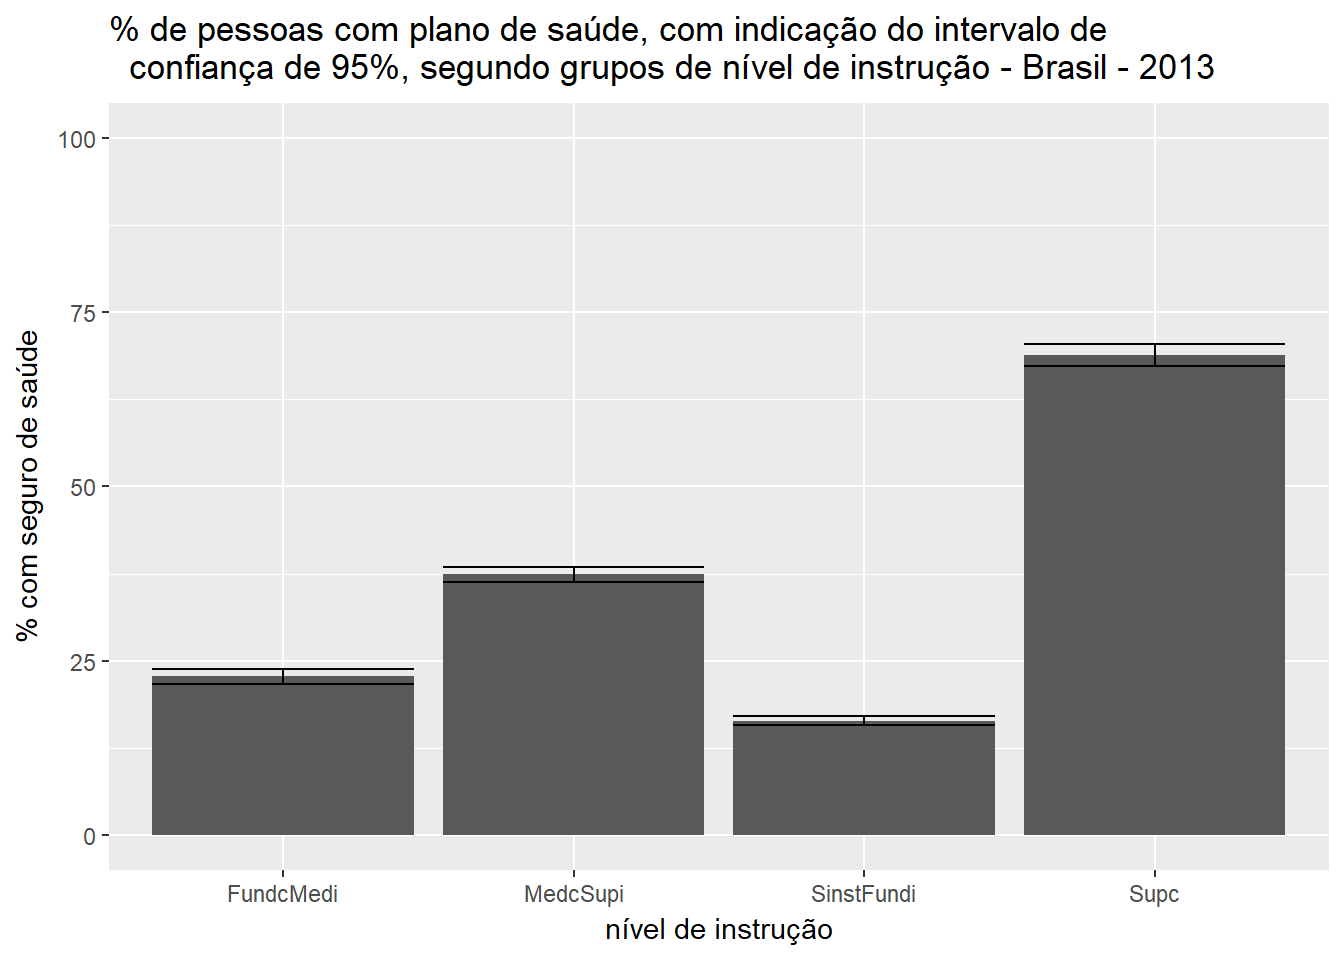
\includegraphics{bookdown-demo_files/figure-latex/unnamed-chunk-60-1.pdf}

\chapter{Referencial para Inferência}\label{refinf}

\chapter{Estimação Baseada no Plano Amostral}\label{capplanamo}

\chapter{Efeitos do Plano Amostral}\label{epa}

\chapter{Ajuste de Modelos Paramétricos}\label{ajmodpar}

\chapter{Modelos de Regressão}\label{modreg}

\chapter{Testes de Qualidade de Ajuste}\label{testqualajust}

\chapter{Testes em Tabelas de Duas Entradas}\label{testetab2}

\chapter{Estimação de densidades}\label{estimacao-de-densidades}

\chapter{Modelos Hierárquicos}\label{modelos-hierarquicos}

\chapter{Não-Resposta}\label{nao-resposta}

\chapter{Diagnóstico de ajuste de
modelo}\label{diagnostico-de-ajuste-de-modelo}

\chapter{Agregação vs.~Desagregação}\label{agregdesag}

\chapter{Pacotes para Analisar Dados Amostrais}\label{pacotes}

\chapter{Placeholder}\label{placeholder}

\chapter{Placeholder}\label{placeholder-1}

\bibliography{packages,book}


\end{document}
